\documentclass{article}
\usepackage[margin=1in]{geometry}
\usepackage{setspace}
\usepackage{amsmath}
\usepackage{amssymb}
\usepackage{physics}
\usepackage{graphicx}
\usepackage{relsize}

\title{Math 132 Midterm 1}
\author{Jiaping Zeng}
\date{10/26/2020}

\begin{document}
\setstretch{1.5}

\newpage
\begin{itemize}
    \item [P2] $(z-2-2i)^4=16i$\\
          \textbf{Answer}: Let $w=z-2-2i$, then we have $w^4=16i\implies w^4=16(\cos\frac{\pi}{2}+i\sin\frac{\pi}{2})$. Then by the $n$th roots formula, the roots are:\\
          $w_1=\sqrt[4]{16}\left[\cos(\frac{1}{4}\cdot\frac{\pi}{2})+i\sin(\frac{1}{4}\cdot\frac{\pi}{2})\right]=2(\cos\frac{\pi}{8}+i\sin\frac{\pi}{8})$\\
          $w_2=\sqrt[4]{16}\left[\cos(\frac{1}{4}\cdot\frac{\pi}{2}+\frac{\pi}{2})+i\sin(\frac{1}{4}\cdot\frac{\pi}{2}+\frac{\pi}{2})\right]=2(\cos\frac{5\pi}{8}+i\sin\frac{5\pi}{8})$\\
          $w_3=\sqrt[4]{16}\left[\cos(\frac{1}{4}\cdot\frac{\pi}{2}+\pi)+i\sin(\frac{1}{4}\cdot\frac{\pi}{2}+\pi)\right]=2(\cos\frac{9\pi}{8}+i\sin\frac{9\pi}{8})$\\
          $w_4=\sqrt[4]{16}\left[\cos(\frac{1}{4}\cdot\frac{\pi}{2}+\frac{3\pi}{2})+i\sin(\frac{1}{4}\cdot\frac{\pi}{2}+\frac{3\pi}{2})\right]=2(\cos\frac{13\pi}{8}+i\sin\frac{13\pi}{8})$\\
          By substitution we have:\\
          $z_1=w_1+2+2i=(2+2\cos\frac{\pi}{8})+(2+2\sin\frac{\pi}{8})i$\\
          $z_2=w_2+2+2i=(2+2\cos\frac{5\pi}{8})+(2+2\sin\frac{5\pi}{8})i$\\
          $z_3=w_3+2+2i=(2+2\cos\frac{9\pi}{8})+(2+2\sin\frac{9\pi}{8})i$\\
          $z_4=w_4+2+2i=(2+2\cos\frac{13\pi}{8})+(2+2\sin\frac{13\pi}{8})i$
          \begin{center}
              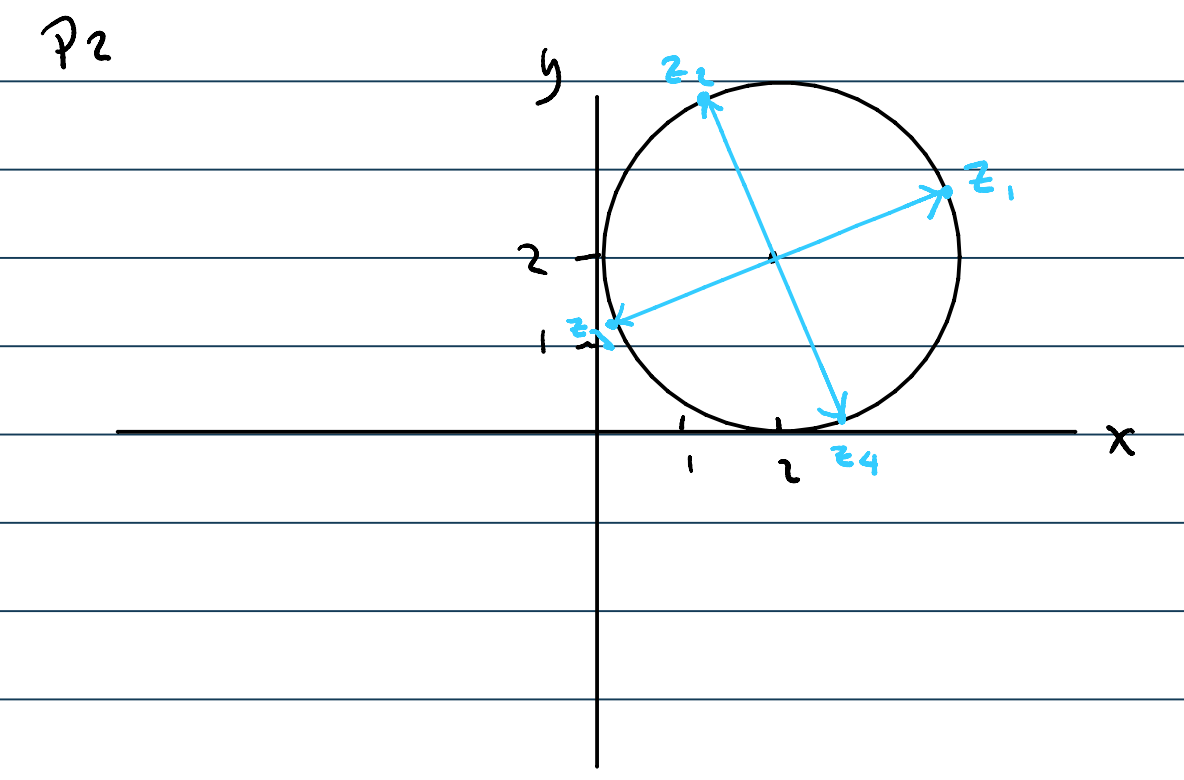
\includegraphics[width=6in]{p2.png}
          \end{center}
\end{itemize}

\newpage
\begin{itemize}
    \item [P3] Let $\gamma$ be the pictured path, consisting of an arc of the circle of radius $2$ centered at $0$, joined with the line segment $[2i,3+2i]$.
          \begin{center}
              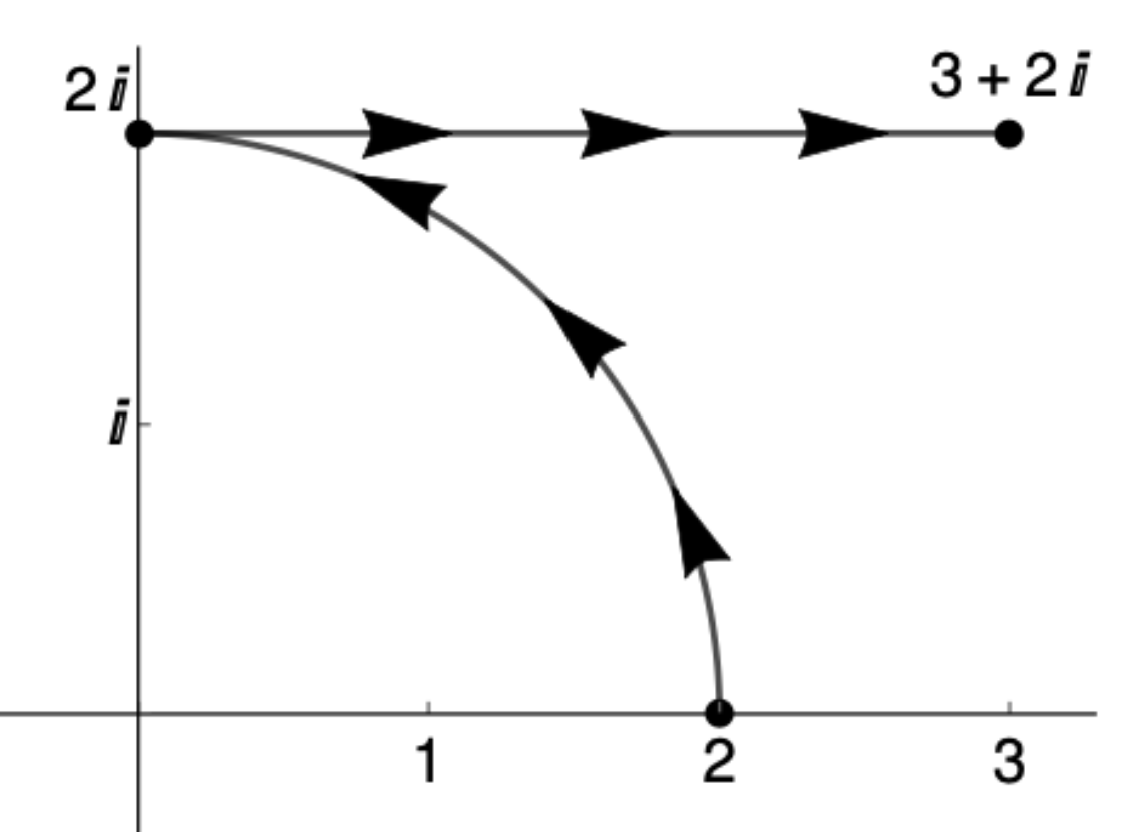
\includegraphics[width=3in]{p3.png}
          \end{center}
          Evaluate $\mathlarger{\int_\gamma(\bar{z}+2i)dz}$.\\
          \textbf{Answer}: Let $\gamma_1$ be the arc and $\gamma_2$ be the line segment, then $\gamma_1(t)=2e^{it}, t\in[0,\frac{\pi}{2}]$ and $\gamma_2(t)=2i+3t, t\in[0,1]$. In addition, we have $\gamma_1'(t)=2ie^{it}$ and $\gamma_2'(t)=3$.\\
          $\mathlarger{\int_\gamma(\bar{z}+2i)dz}$\\
          $=\mathlarger{\int_{\gamma_1}(\bar{z}+2i)dz+\int_{\gamma_2}(\bar{z}+2i)dz}$\\
          $=\mathlarger{\int_{0}^{\frac{\pi}{2}}[\overline{\gamma_1(t)}+2i]\gamma_1'(t)dt+\int_{0}^{1}[\overline{\gamma_2(t)}+2i]\gamma_2'(t)dt}$\\
          $=\mathlarger{\int_{0}^{\frac{\pi}{2}}2ie^{it}(2e^{-it}+2i)dt}+\int_{0}^{1}3(3t-2i+2i)dt$\\
          $=\mathlarger{\int_{0}^{\frac{\pi}{2}}4i-4e^{it}dt+\int_{0}^{1}9tdt}$\\
          $=4\mathlarger{\int_{0}^{\frac{\pi}{2}}idt-4\int_{0}^{\frac{\pi}{2}}e^{it}dt+9\int_{0}^{1}tdt}$\\
          $=4[it]_{0}^{\frac{\pi}{2}}+4[ie^{it}]_{0}^{\frac{\pi}{2}}+9[\frac{t^2}{2}]_0^1$\\
          $=2\pi i+4(ie^{\frac{\pi}{2}i}-i)+\frac{9}{2}$\\
          $=\frac{9}{2}+i(2\pi-4+4e^{\frac{\pi}{2}i})$
\end{itemize}

\newpage
\begin{itemize}
    \item [P4]
          \begin{itemize}
              \item [(a)] Show that $\abs{e^z}\leq e^{\abs{z}}$ for all $z\in\mathbb{C}$.\\
              \textbf{Answer}: Let $z=x+iy$, we have $\abs{e^z}=\abs{e^{x+iy}}=\abs{e^x\cdot e^{iy}}=\abs{e^x}\cdot\abs{e^{iy}}=e^x$; then since $x=\Re z\leq\abs{z}$, we have $e^x\leq e^{\abs{z}}$. Therefore $\abs{e^z}=e^x\leq e^{\abs{z}}\implies\abs{e^z}\leq e^{\abs{z}}$.
              \item [(b)] Show that $\abs{\cos z}\leq e^{\abs{z}}$ for all $z\in\mathbb{C}$.\\
              \textbf{Answer}: By definition, $\cos z=\frac{1}{2}(e^{iz}+e^{-iz})=\frac{1}{2}(e^{i(x+iy)}+e^{-i(x+iy)})=\frac{1}{2}(e^{-y+ix}+e^{y-ix})$, then $\abs{\cos z}=\frac{1}{2}\abs{e^{-y+ix}+e^{y-ix}}=\frac{1}{2}\abs{e^{-y}\cdot e^{ix}+e^{y}\cdot e^{-ix}}$. Using triangle inequality, we have $\frac{1}{2}\abs{e^{-y}\cdot e^{ix}+e^{y}\cdot e^{-ix}}\leq\frac{1}{2}\abs{e^{-y}\cdot e^{ix}}+\frac{1}{2}\abs{e^{y}\cdot e^{-ix}}=\frac{1}{2}\abs{e^{-y}}\cdot\abs{e^{ix}}+\frac{1}{2}\abs{e^{y}}\cdot\abs{e^{-ix}}=\frac{1}{2}\abs{e^{-y}}+\frac{1}{2}\abs{e^{y}}$. By part (a), $\frac{1}{2}\abs{e^{-y}}+\frac{1}{2}\abs{e^{y}}\leq\frac{1}{2}e^{\abs{-y}}+\frac{1}{2}e^{\abs{y}}=e^{\abs{y}}$. Then $\abs{\cos z}\leq e^{\abs{y}}\leq e^{\abs{z}}\implies\abs{\cos z}\leq e^{\abs{z}}$.
              \item [(c)] Show that $\abs{\frac{e^z\cos z}{z-i}}\leq\frac{e^{10}}{2}$ for all $z$ on $C_3(2i)$.\\
              \textbf{Answer}: Since $\abs{\frac{e^z\cos z}{z-i}}=\frac{\abs{e^z}\cdot\abs{\cos z}}{\abs{z-i}}$, we can apply parts (a) and (b) which gives us $\frac{\abs{e^z}\cdot\abs{\cos z}}{\abs{z-i}}\leq\frac{e^{2\abs{z}}}{\abs{z-i}}$. To show that the given inequality is true, we will show that $e^{2\abs{z}}\leq e^{10}$ and $\abs{z-i}\geq 2$ separately.\\
              On the numerator, we want to show that $e^{2\abs{z}}\leq e^{10}$; since $\abs{z}\geq 0$, it is sufficient to show that $2\abs{z}\leq 10$, or $\abs{z}\leq 5$. Since we are only considering $z\in C_3(2i)\implies\abs{z-2i}=3$, by triangle inequality we have $\abs{z}=\abs{(z-2i)+2i}\leq\abs{z-2i}+\abs{2i}=3+2=5\implies\abs{z}\leq 5$.\\
              On the denominator we have $\abs{z-i}=\abs{(z-2i)+i}\geq\abs{\abs{z-2i}-\abs{i}}$ by triangle inequality; since $z\in C_3(2i)\implies\abs{z-2i}=3$, we then have $\abs{\abs{z-2i}-\abs{i}}=\abs{3-1}=2$. So $\abs{z-i}\geq 2$.\\
              As shown above, we have $e^{2\abs{z}}\leq e^{10}$ and $\abs{z-i}\geq 2$, therefore $\abs{\frac{e^z\cos z}{z-i}}=\frac{\abs{e^z}\cdot\abs{\cos z}}{\abs{z-i}}\leq\frac{e^{2\abs{z}}}{\abs{z-i}}\leq\frac{e^{10}}{2}\implies\abs{\frac{e^z\cos z}{z-i}}\leq\frac{e^{10}}{2}$.
          \end{itemize}
\end{itemize}

\newpage
I certify on my honor that I have neither given nor received any help, or used any non-permitted resources, while completing this evaluation.\\
Signature:
\includegraphics[width=2in]{signature.png}\\
Date: 10/26/2020


\end{document}